%%%%%%%%%%%%%%%%%%%%%%%%%%%%%%%%%%%%%%%%%%%%%%%%%%%%%%%%%%%%%%%%%%%%%%%%%%%%%%%%
% TUM-Vorlage: Präsentation
%%%%%%%%%%%%%%%%%%%%%%%%%%%%%%%%%%%%%%%%%%%%%%%%%%%%%%%%%%%%%%%%%%%%%%%%%%%%%%%%
%
% Rechteinhaber:
%     Technische Universität München
%     https://www.tum.de
% 
% Gestaltung:
%     ediundsepp Gestaltungsgesellschaft, München
%     http://www.ediundsepp.de
% 
% Technische Umsetzung:
%     eWorks GmbH, Frankfurt am Main
%     http://www.eworks.de
%
%%%%%%%%%%%%%%%%%%%%%%%%%%%%%%%%%%%%%%%%%%%%%%%%%%%%%%%%%%%%%%%%%%%%%%%%%%%%%%%%


%%%%%%%%%%%%%%%%%%%%%%%%%%%%%%%%%%%%%%%%%%%%%%%%%%%%%%%%%%%%%%%%%%%%%%%%%%%%%%%%
% Zur Wahl des Seitenverhältnisses bitte einen der beiden folgenden Befehle
% auskommentieren und den ausführen lassen:
\input{Praeambel4zu3.tex} % Seitenverhältnis 4:3
% \input{./Ressourcen/Praesentation/Praeambel16zu9.tex} % Seitenverhältnis 16:9
%%%%%%%%%%%%%%%%%%%%%%%%%%%%%%%%%%%%%%%%%%%%%%%%%%%%%%%%%%%%%%%%%%%%%%%%%%%%%%%%


%%%%%%%%%%%%%%%%%%%%%%%%%%%%%%%%%%%%%%%%%%%%%%%%%%%%%%%%%%%%%%%%%%%%%%%%%%%%%%%%
%%%%%%%%%%%%%%%%%%%%%%%%%%%%%%%%%%%%%%%%%%%%%%%%%%%%%%%%%%%%%%%%%%%%%%%%%%%%%%%%
% TUM-Vorlage: Personenspezifische Informationen
%%%%%%%%%%%%%%%%%%%%%%%%%%%%%%%%%%%%%%%%%%%%%%%%%%%%%%%%%%%%%%%%%%%%%%%%%%%%%%%%
%
% Rechteinhaber:
%     Technische Universität München
%     https://www.tum.de
% 
% Gestaltung:
%     ediundsepp Gestaltungsgesellschaft, München
%     http://www.ediundsepp.de
% 
% Technische Umsetzung:
%     eWorks GmbH, Frankfurt am Main
%     http://www.eworks.de
%
%%%%%%%%%%%%%%%%%%%%%%%%%%%%%%%%%%%%%%%%%%%%%%%%%%%%%%%%%%%%%%%%%%%%%%%%%%%%%%%%

% Für die Person anpassen:

\newcommand{\PersonVorname}{Raffael}
\newcommand{\PersonNachname}{D\"ull}
\newcommand{\PersonStadt}{Munich}
\newcommand{\PersonAdresse}{}
\newcommand{\PersonTelefon}{}
\newcommand{\PersonFax}{}
\newcommand{\PersonEmail}{raffael.duell@tum.de}
\newcommand{\PersonWebseite}{}

\newcommand{\FakultaetAnsprechpartner}{}
% Fakultät:
\newcommand{\FakultaetName}{Faculty for Informatics}
\newcommand{\LehrstuhlName}{}

\newcommand{\EinstellungBankName}{}
\newcommand{\EinstellungBankIBAN}{}
\newcommand{\EinstellungBankBIC}{}
\newcommand{\EinstellungSteuernummer}{}
\newcommand{\EinstellungUmsatzsteuerIdentifikationsnummer}{}

\hyphenation{} % eigene Silbentrennung                    % !!! DATEI ANPASSEN !!!
%%%%%%%%%%%%%%%%%%%%%%%%%%%%%%%%%%%%%%%%%%%%%%%%%%%%%%%%%%%%%%%%%%%%%%%%%%%%%%%%

\usepackage{amsmath}
\usepackage{bm}
\definecolor{princetonorange}{rgb}{1.0, 0.56, 0.0}
\newcommand{\Datum}{\today}

\renewcommand{\PraesentationFusszeileZusatz}{| Seminar WaveSim | Topic 8: Source terms}

\title{Topic 8: Source terms}
\author{\PersonTitel{} \PersonVorname{} \PersonNachname}
\institute[]{\UniversitaetName \\ \FakultaetName \\ \LehrstuhlName}
\date[\Datum]{Munich, 30 January 2020}
\subject{Thema der Präsentation}


%%%%%%%%%%%%%%%%%%%%%%%%%%%%%%%%%%%%%%%%%%%%%%%%%%%%%%%%%%%%%%%%%%%%%%%%%%%%%%%%
\input{Anfang.tex} % !!! NICHT ENTFERNEN !!!
\begin{document}
\setlength{\baselineskip}{\PraesentationAbstandAbsatz}
\setlength{\parskip}{\baselineskip}
%%%%%%%%%%%%%%%%%%%%%%%%%%%%%%%%%%%%%%%%%%%%%%%%%%%%%%%%%%%%%%%%%%%%%%%%%%%%%%%%


%%%%%%%%%%%%%%%%%%%%%%%%%%%%%%%%%%%%%%%%%%%%%%%%%%%%%%%%%%%%%%%%%%%%%%%%%%%%%%%%
% FOLIENSTIL: Standard
% !!!ÄNDERUNG HIER:!!!
\PraesentationMasterStandard


%%%%%%%%%%%%%%%%%%%%%%%%%%%%%%%%%%%%%%%%%%%%%%%%%%%%%%%%%%%%%%%%%%%%%%%%%%%%%%%%
% FOLIENSTIL: Standard mit Lehrstuhl-, Fakultäts- und Universitätsnamen im
% Kopfbereich links
\PraesentationMasterKopfzeileDreizeiler

%%%%%%%%%%%%%%%%%%%%%%%%%%%%%%%%%%%%%%%%%%%%%%%%%%%%%

\PraesentationTitelseite % Fügt die Startseite ein


\begin{frame}
    \frametitle{Burgers Equation}
    
We consider the Burgers equation with source term:
\begin{equation*}
	\frac{\partial q}{\partial t} + \underbrace{\frac{1}{2}\frac{\partial q^2}{\partial x}}_{transport} = \underbrace{\vphantom{\frac{\partial q}{\partial t}}\psi (q,x)}_{source}
	\label{eq:system}
\end{equation*}

\vspace{0.6cm}
\begin{multicols}{2}
    \centering
    Operator ${\color{red}\bm{\mathcal{A}}}$ for the transport term: 
    \begin{equation*}
        {\color{red}\bm{\mathcal{A}}}q = - \frac{1}{2}\frac{\partial q^2}{\partial x}
    \end{equation*}
    Operator ${\color{blue}\bm{\mathcal{B}}}$ for the source term: 
    \begin{equation*}
        {\color{blue}\bm{\mathcal{B}}}q = \psi (q,x)
    \end{equation*}
\end{multicols}

\vspace{0.6cm}
\pause
We can rewrite the problem to the form: 
\begin{equation*}
	\frac{\partial q}{\partial t} = ({\color{red}\bm{\mathcal{A}}} + {\color{blue}\bm{\mathcal{B}}}) q 	
	\label{eq:generalPDE}
\end{equation*}

The idea of splitting methods is to solve for ${\color{red}\bm{\mathcal{A}}}$ and ${\color{blue}\bm{\mathcal{B}}}$ independently.

\end{frame}






\begin{frame}
    \frametitle{Godunov Splitting}
\begin{itemize}
    \item For classical \textbf{unsplit methods}, we look for a numerical scheme $\color{princetonorange}\bm{\mathcal{C}_{\Delta t}}$ which directly approximates $({\color{red}\bm{\mathcal{A}}} + {\color{blue}\bm{\mathcal{B}}}) q$
    \begin{equation*}
    	\frac{\partial q}{\partial t} = \underbrace{({\color{red}\bm{\mathcal{A}}} + {\color{blue}\bm{\mathcal{B}}}) q}_{{\color{princetonorange}\bm{\mathcal{C}}}q} \qquad \xrightarrow{} \qquad Q(t+\Delta t) = {\color{princetonorange}\bm{\mathcal{C}_{\Delta t}}}Q(t)
    \end{equation*}
\pause
    \item For \textbf{Godunov splitting}, we first apply the operator ${\color{red}\bm{\mathcal{A}}}$ then ${\color{blue}\bm{\mathcal{B}}}$
    \begin{equation*}
    	\frac{\partial q}{\partial t} = {\color{blue}\bm{\mathcal{B}}} ({\color{red}\bm{\mathcal{A}}} q)
    \end{equation*}
    It is now enough to only consider the two subproblems: 
    \begin{equation*}
    	\frac{\partial q^*}{\partial t} = {\color{red}\bm{\mathcal{A}}} q^* \qquad \text{and} \qquad \frac{\partial q^{**}}{\partial t} = {\color{blue}\bm{\mathcal{B}}} q^{**}
    \end{equation*}
    for which we can find the numerical schemes ${\color{red}\bm{\mathcal{A}_{\Delta t}}}$ and ${\color{blue}\bm{\mathcal{B}_{\Delta t}}}$
    \begin{equation*}
        Q^*(t+\Delta t) = {\color{red}\bm{\mathcal{A}_{\Delta t}}}Q^*(t) \qquad \text{and} \qquad Q^{**}(t+\Delta t) = {\color{blue}\bm{\mathcal{B}_{\Delta t}}}Q^{**}(t)
    \end{equation*}{}

\end{itemize}{}
\end{frame}






\begin{frame}{}
    \frametitle{Godunov Splitting}
    To implement this scheme, we alternate ${\color{red}\bm{\mathcal{A}_{\Delta t}}}$ and $ {\color{blue}\bm{\mathcal{B}_{\Delta t}}}$. In each time step we apply: 
    \begin{itemize}
        \item First step: $\quad Q^*(t + \Delta t) = {\color{red}\bm{\mathcal{A}_{\Delta t}}}Q(t)$ 
        \item Second step: $Q(t + \Delta t) &= {\color{blue}\bm{\mathcal{B}_{\Delta t}}}Q^*(t+\Delta t)$ \pause
    \end{itemize}{}
    No error if ${\color{red}\bm{\mathcal{A}}}$ and ${\color{blue}\bm{\mathcal{B}}}$ commute! $\quad \Leftrightarrow \quad {\color{blue}\bm{\mathcal{B}}} ({\color{red}\bm{\mathcal{A}}} q) = {\color{red}\bm{\mathcal{A}}} ({\color{blue}\bm{\mathcal{B}}} q)$ \newline
    In the general case the error is of the order $\mathcal{O}(\Delta t)$ \newline 
    BUT... \\
    The accuracy of the method is decreased if the solvers ${\color{red}\bm{\mathcal{A}}}$ and ${\color{blue}\bm{\mathcal{B}}}$ are of second order (or higher). \newline
    We need a fractional step method of higher order!

\end{frame}





\begin{frame}
     \frametitle{Strang Splitting}
     In \textbf{Strang splitting}, we apply ${\color{red}\bm{\mathcal{A}_\frac{\Delta t}{2}}}$ for half a time step before and after $ {\color{blue}\bm{\mathcal{B}_{\Delta t}}}$. Thus:
    \begin{itemize}
        \item First step: $\quad\ \ \ Q^*(t + \frac{\Delta t}{2}) = {\color{red}\bm{\mathcal{A}_\frac{\Delta t}{2}}}Q(t)$ 
        \item Second step: $\: Q^{**}(t + \frac{\Delta t}{2}) = {\color{blue}\bm{\mathcal{B}_{\Delta t}}}Q^*(t+\frac{\Delta t}{2})$
        \item Third step: $\qquad Q(t + \Delta t) = {\color{red}\bm{\mathcal{A}_\frac{\Delta t}{2}}}Q^{**}(t+\frac{\Delta t}{2})$ \pause

    \end{itemize}{}
     In the general case the error is of the order $\mathcal{O}(\Delta t^2)$ \newline
     In practice, Godunov and Strang splitting yield very similar results despite the theoretical difference. 


\end{frame}{}



\begin{frame}{}
    \frametitle{An Example of a Stiff Source Term}
    \begin{equation*}
        	 \frac{\partial q}{\partial t} + \frac{1}{2}\frac{\partial q^2}{\partial x}= \bm{\frac{1}{\tau} q (q - \beta)(1 - q)}
    \end{equation*}
    \begin{multicols}{2}
        . \\
        Stable equilibrium at $q=0$ and $q=1$ \\
        Unstable equilibrium at $q=\beta$ \\ 
        $\tau$ regulates the stiffness  \\ \vspace{1cm} 
        Boundaries: 0 to the left, 1 to the right \\
        Rarefaction wave as homogeneous solution \\
        Wave travels with speed $\beta$ to the right
        \pause
    \begin{figure}[!h]
    \centering
     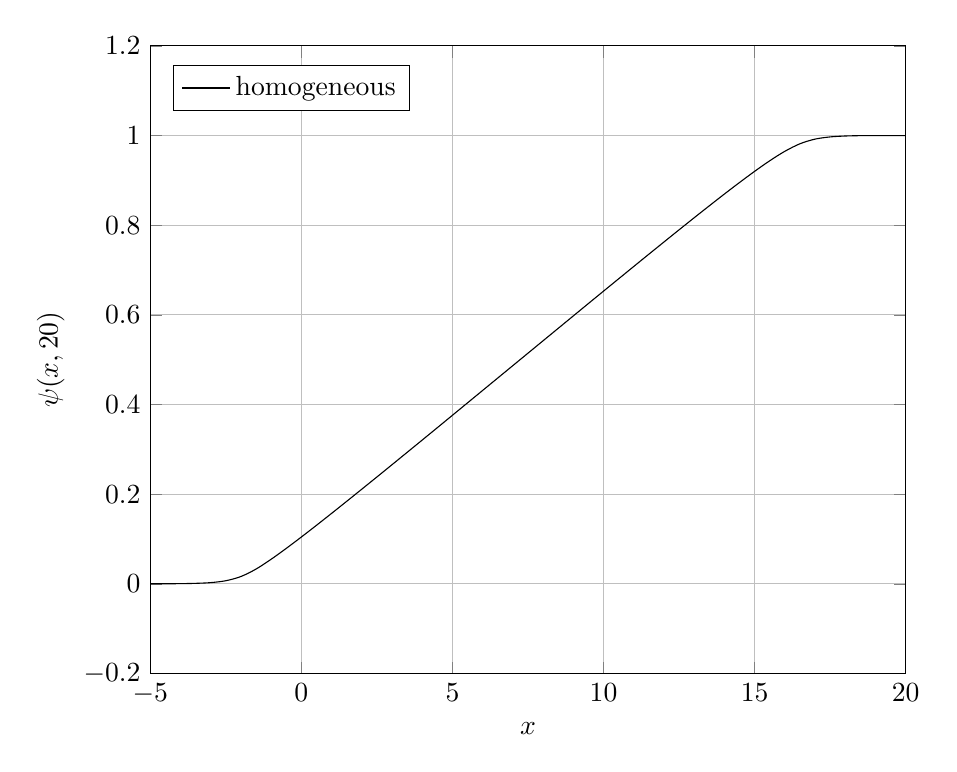
\begin{tikzpicture}
       \begin{axis}[grid=major, xmin=-5, xmax=20, ymin=-0.2, ymax=1.2,
         xlabel=$x$, ylabel={$\psi(x,20)$}, legend pos=north west,
         xtick = {-5,0,...,20}, ytick = {-0.2,0,...,1.2},
         scale=1.4]
         \addplot[black, smooth]
           plot coordinates {
           (-5, 0.0001)    
           (-4.5, 0.0001)
           (-4, 0.0003)
           (-3.5, 0.0010)
           (-3, 0.0026)
           (-2.5, 0.0068)
           (-2, 0.0162)
           (-1.5, 0.0328)
           (-1, 0.0547)
           (-0.5, 0.0789)
           (0, 0.1043)
           (0.5, 0.1304)
           (1, 0.1570)
           (1.5, 0.1839)
           (2, 0.2110)
           (2.5, 0.2382)
           (3, 0.2656)
           (3.5, 0.2931)
           (4, 0.3206)
           (4.5, 0.3482)
           (5, 0.3759)
           (5.5, 0.4036)
           (6, 0.4313)
           (6.5, 0.4590)
           (7, 0.4867)
           (7.5, 0.5144)
           (8, 0.5421)
           (8.5, 0.5698)
           (9, 0.5975)
           (9.5, 0.6252)
           (10, 0.6528)
           (10.5, 0.6803)
           (11, 0.7078)
           (11.5, 0.7352)
           (12, 0.7624)
           (12.5, 0.7896)
           (13, 0.8165)
           (13.5, 0.8431)
           (14, 0.8694)
           (14.5, 0.8951)
           (15, 0.9200)
           (15.5, 0.9436)
           (16, 0.9647)
           (16.5, 0.9815)
           (17, 0.9919) 
           (17.5, 0.9968)
           (18, 0.9988)
           (18.5, 0.9996)
           (19, 0.9998)
           (19.5, 0.9998)
           (20, 0.9998)
           };
         \addlegendentry{homogeneous} 
       \end{axis}
    \end{tikzpicture}
    \caption{Analytical solution after 20s}
    \label{fig:honesty}
    \end{figure}
    \end{multicols}
\end{frame}{}





\begin{frame}[noframenumbering]
    \frametitle{An Example of a Stiff Source Term}
    \begin{equation*}
        	 \frac{\partial q}{\partial t} + \frac{1}{2}\frac{\partial q^2}{\partial x}= \bm{\frac{1}{\tau} q (q - \beta)(1 - q)}
    \end{equation*}
    \begin{multicols}{2}
        . \\
        Stable equilibrium at $q=0$ and $q=1$ \\
        Unstable equilibrium at $q=\beta$ \\ 
        $\tau$ regulates the stiffness  \\ \vspace{1cm} 
        Boundaries: 0 to the left, 1 to the right \\
        Rarefaction wave as homogeneous solution \\
        Wave travels with speed $\beta$ to the right
    \begin{figure}[!h]
    \centering
     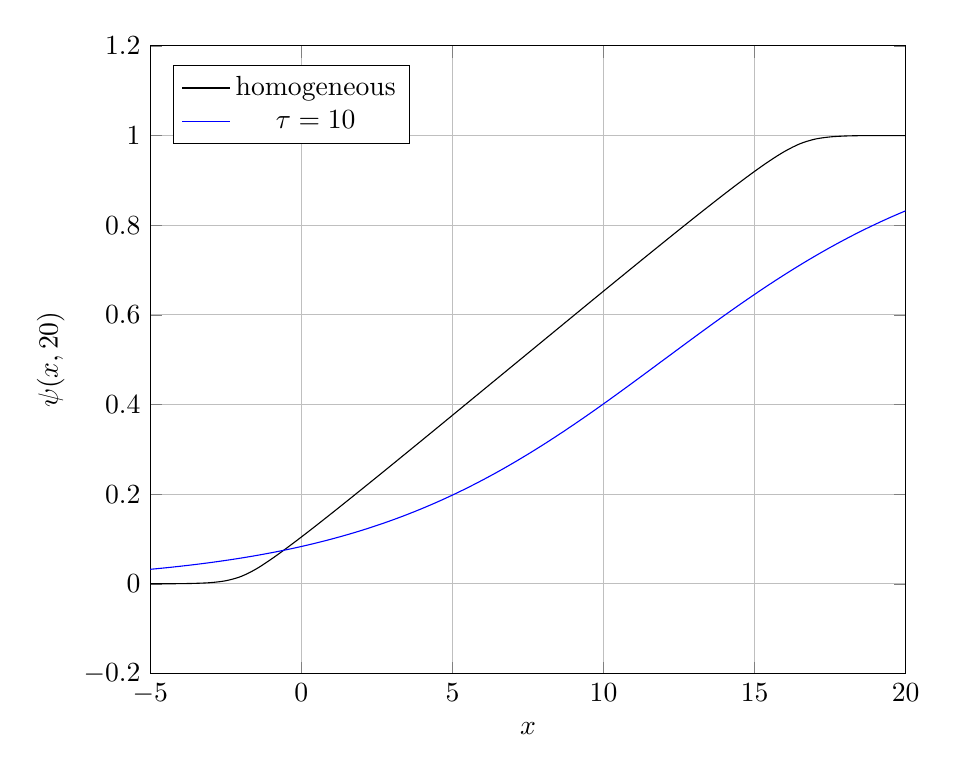
\begin{tikzpicture}
       \begin{axis}[grid=major, xmin=-5, xmax=20, ymin=-0.2, ymax=1.2,
         xlabel=$x$, ylabel={$\psi(x,20)$}, legend pos=north west,
         xtick = {-5,0,...,20}, ytick = {-0.2,0,...,1.2},
         scale=1.4]
         \addplot[black, smooth]
           plot coordinates {
           (-5, 0.0001)    
           (-4.5, 0.0001)
           (-4, 0.0003)
           (-3.5, 0.0010)
           (-3, 0.0026)
           (-2.5, 0.0068)
           (-2, 0.0162)
           (-1.5, 0.0328)
           (-1, 0.0547)
           (-0.5, 0.0789)
           (0, 0.1043)
           (0.5, 0.1304)
           (1, 0.1570)
           (1.5, 0.1839)
           (2, 0.2110)
           (2.5, 0.2382)
           (3, 0.2656)
           (3.5, 0.2931)
           (4, 0.3206)
           (4.5, 0.3482)
           (5, 0.3759)
           (5.5, 0.4036)
           (6, 0.4313)
           (6.5, 0.4590)
           (7, 0.4867)
           (7.5, 0.5144)
           (8, 0.5421)
           (8.5, 0.5698)
           (9, 0.5975)
           (9.5, 0.6252)
           (10, 0.6528)
           (10.5, 0.6803)
           (11, 0.7078)
           (11.5, 0.7352)
           (12, 0.7624)
           (12.5, 0.7896)
           (13, 0.8165)
           (13.5, 0.8431)
           (14, 0.8694)
           (14.5, 0.8951)
           (15, 0.9200)
           (15.5, 0.9436)
           (16, 0.9647)
           (16.5, 0.9815)
           (17, 0.9919) 
           (17.5, 0.9968)
           (18, 0.9988)
           (18.5, 0.9996)
           (19, 0.9998)
           (19.5, 0.9998)
           (20, 0.9998)
           };
         \addlegendentry{homogeneous} 
         \addplot[blue, samples=100, domain=-5:20, smooth, unbounded coords=discard]
           plot (\x, { 0.5 * (1 + tanh((x - 0.6 * 20) / 10)) });
         \addlegendentry{$\tau=10$} 
       \end{axis}
    \end{tikzpicture}
    \caption{Analytical solution after 20s}
    \label{fig:honesty}
    \end{figure}
    \end{multicols}
\end{frame}{}




\begin{frame}[noframenumbering]
    \frametitle{An Example of a Stiff Source Term}
    \begin{equation*}
        	 \frac{\partial q}{\partial t} + \frac{1}{2}\frac{\partial q^2}{\partial x}= \bm{\frac{1}{\tau} q (q - \beta)(1 - q)}
    \end{equation*}
    \begin{multicols}{2}
        . \\
        Stable equilibrium at $q=0$ and $q=1$ \\
        Unstable equilibrium at $q=\beta$ \\ 
        $\tau$ regulates the stiffness  \\ \vspace{1cm} 
        Boundaries: 0 to the left, 1 to the right \\
        Rarefaction wave as homogeneous solution \\
        Wave travels with speed $\beta$ to the right
    \begin{figure}[!h]
    \centering
     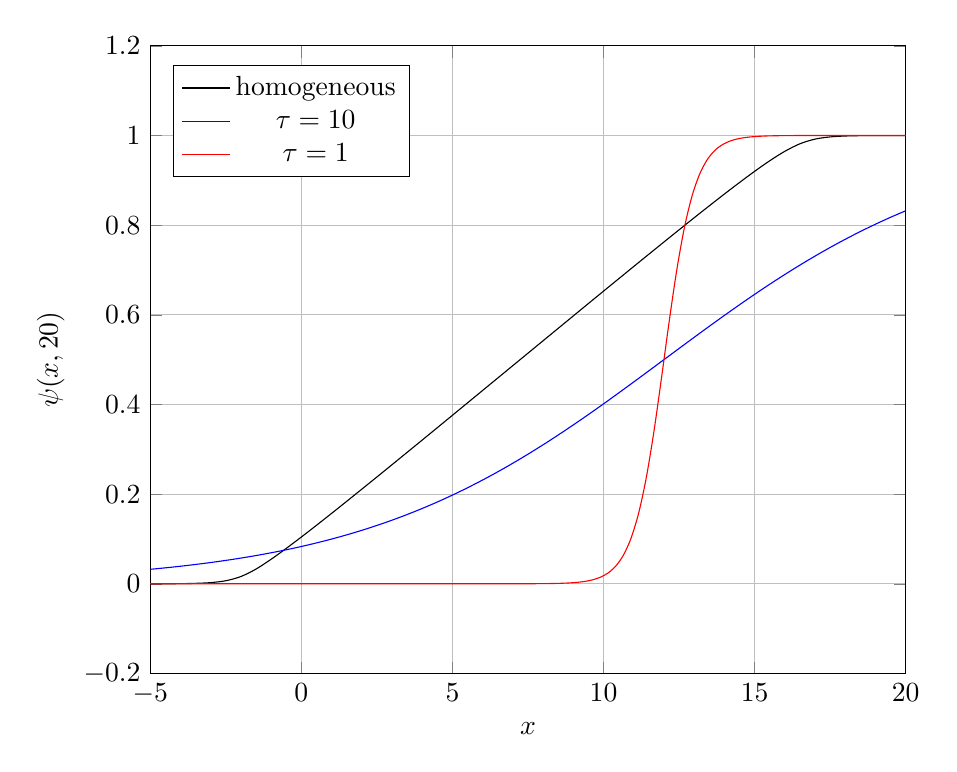
\begin{tikzpicture}
       \begin{axis}[grid=major, xmin=-5, xmax=20, ymin=-0.2, ymax=1.2,
         xlabel=$x$, ylabel={$\psi(x,20)$}, legend pos=north west,
         xtick = {-5,0,...,20}, ytick = {-0.2,0,...,1.2},
         scale=1.4]
         \addplot[black, smooth]
           plot coordinates {
           (-5, 0.0001)    
           (-4.5, 0.0001)
           (-4, 0.0003)
           (-3.5, 0.0010)
           (-3, 0.0026)
           (-2.5, 0.0068)
           (-2, 0.0162)
           (-1.5, 0.0328)
           (-1, 0.0547)
           (-0.5, 0.0789)
           (0, 0.1043)
           (0.5, 0.1304)
           (1, 0.1570)
           (1.5, 0.1839)
           (2, 0.2110)
           (2.5, 0.2382)
           (3, 0.2656)
           (3.5, 0.2931)
           (4, 0.3206)
           (4.5, 0.3482)
           (5, 0.3759)
           (5.5, 0.4036)
           (6, 0.4313)
           (6.5, 0.4590)
           (7, 0.4867)
           (7.5, 0.5144)
           (8, 0.5421)
           (8.5, 0.5698)
           (9, 0.5975)
           (9.5, 0.6252)
           (10, 0.6528)
           (10.5, 0.6803)
           (11, 0.7078)
           (11.5, 0.7352)
           (12, 0.7624)
           (12.5, 0.7896)
           (13, 0.8165)
           (13.5, 0.8431)
           (14, 0.8694)
           (14.5, 0.8951)
           (15, 0.9200)
           (15.5, 0.9436)
           (16, 0.9647)
           (16.5, 0.9815)
           (17, 0.9919) 
           (17.5, 0.9968)
           (18, 0.9988)
           (18.5, 0.9996)
           (19, 0.9998)
           (19.5, 0.9998)
           (20, 0.9998)
           };
         \addlegendentry{homogeneous} 
         \addplot[blue, samples=100, domain=-5:20, smooth, unbounded coords=discard]
           plot (\x, { 0.5 * (1 + tanh((x - 0.6 * 20) / 10)) });
         \addlegendentry{$\tau=10$} 
         \addplot[red, samples=100, domain=-5:20, smooth, unbounded coords=discard]
           plot (\x, { 0.5 * (1 + tanh((x - 0.6 * 20) / 1)) });
         \addlegendentry{$\tau=1$} 
         \end{axis}
    \end{tikzpicture}
    \caption{Analytical solution after 20s}
    \label{fig:honesty}
    \end{figure}
    \end{multicols}
\end{frame}{}





\begin{frame}[noframenumbering]
    \frametitle{An Example of a Stiff Source Term}
    \begin{equation*}
        	 \frac{\partial q}{\partial t} + \frac{1}{2}\frac{\partial q^2}{\partial x}= \bm{\frac{1}{\tau} q (q - \beta)(1 - q)}
    \end{equation*}
    \begin{multicols}{2}
        . \\
        Stable equilibrium at $q=0$ and $q=1$ \\
        Unstable equilibrium at $q=\beta$ \\ 
        $\tau$ regulates the stiffness  \\ \vspace{1cm} 
        Boundaries: 0 to the left, 1 to the right \\
        Rarefaction wave as homogeneous solution \\
        Wave travels with speed $\beta$ to the right
    \begin{figure}[!h]
    \centering
     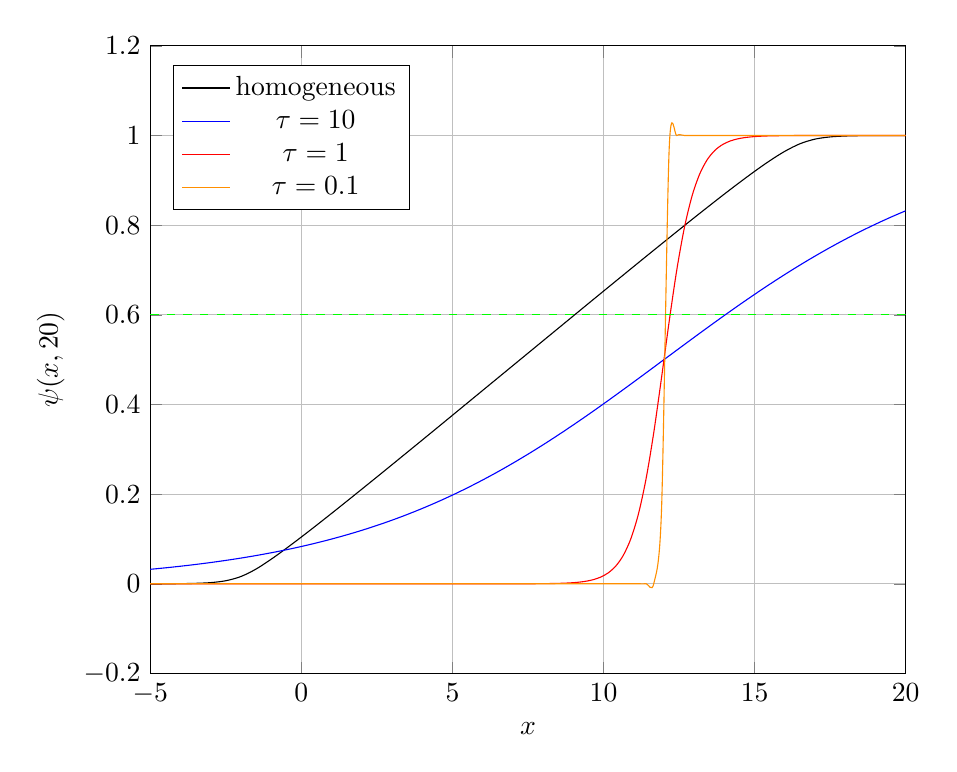
\begin{tikzpicture}
       \begin{axis}[grid=major, xmin=-5, xmax=20, ymin=-0.2, ymax=1.2,
         xlabel=$x$, ylabel={$\psi(x,20)$}, legend pos=north west,
         xtick = {-5,0,...,20}, ytick = {-0.2,0,...,1.2},
         scale=1.4]
         \addplot[black, smooth]
           plot coordinates {
           (-5, 0.0001)    
           (-4.5, 0.0001)
           (-4, 0.0003)
           (-3.5, 0.0010)
           (-3, 0.0026)
           (-2.5, 0.0068)
           (-2, 0.0162)
           (-1.5, 0.0328)
           (-1, 0.0547)
           (-0.5, 0.0789)
           (0, 0.1043)
           (0.5, 0.1304)
           (1, 0.1570)
           (1.5, 0.1839)
           (2, 0.2110)
           (2.5, 0.2382)
           (3, 0.2656)
           (3.5, 0.2931)
           (4, 0.3206)
           (4.5, 0.3482)
           (5, 0.3759)
           (5.5, 0.4036)
           (6, 0.4313)
           (6.5, 0.4590)
           (7, 0.4867)
           (7.5, 0.5144)
           (8, 0.5421)
           (8.5, 0.5698)
           (9, 0.5975)
           (9.5, 0.6252)
           (10, 0.6528)
           (10.5, 0.6803)
           (11, 0.7078)
           (11.5, 0.7352)
           (12, 0.7624)
           (12.5, 0.7896)
           (13, 0.8165)
           (13.5, 0.8431)
           (14, 0.8694)
           (14.5, 0.8951)
           (15, 0.9200)
           (15.5, 0.9436)
           (16, 0.9647)
           (16.5, 0.9815)
           (17, 0.9919) 
           (17.5, 0.9968)
           (18, 0.9988)
           (18.5, 0.9996)
           (19, 0.9998)
           (19.5, 0.9998)
           (20, 0.9998)
           };
         \addlegendentry{homogeneous} 
         \addplot[blue, samples=100, domain=-5:20, smooth, unbounded coords=discard]
           plot (\x, { 0.5 * (1 + tanh((x - 0.6 * 20) / 10)) });
         \addlegendentry{$\tau=10$} 
         \addplot[red, samples=100, domain=-5:20, smooth, unbounded coords=discard]
           plot (\x, { 0.5 * (1 + tanh((x - 0.6 * 20) / 1)) });
         \addlegendentry{$\tau=1$} 
         \addplot[princetonorange, samples=100, domain=-5:20, smooth, unbounded coords=discard]
           plot (\x, { 0.5 * (1 + tanh((x - 0.6 * 20) / 0.1)) });
         \addlegendentry{$\tau=0.1$}
         \addplot[green, dashed, samples=100, domain=-5:20, smooth]
           plot (\x, { 0.6 } );
       \end{axis}
    \end{tikzpicture}
    \caption{Analytical solution after 20s}
    \label{fig:honesty}
    \end{figure}
    \end{multicols}
\end{frame}{}




\begin{frame}
    \frametitle{Implementation}
    Code implemented in MATLAB \\
    Godunov splitting of the 1D Burgers equation with stiff source term  \\ 
    2 solvers for the transport equation and 5 solvers for the source term \\
    Choice of the solver: \\ \pause
    \begin{itemize}
        \item For the transport equation ${\color{red}\bm{\mathcal{A}_{\Delta t}}}$: typical solvers for wave transport (\textbf{Lax-Wendroff} and \textbf{Godunov schemes}) \\
        The \textbf{Godunov scheme} is preferred because it gave better results than \textbf{Lax-Wendroff}. \pause
        \item For the source term equation ${\color{blue}\bm{\mathcal{B}_{\Delta t}}}$: depends a lot on the source $\psi(q,x)$ 
        \begin{itemize}
            \item Direct solver - the easiest, not too much of interest
            \item Explicit schemes - tend to be unstable (e.g. \textbf{explicit Euler}, \textbf{Runge-Kutta 2})
            \item Implicit schemes - usually stable, but expensive to compute (e.g. \textbf{implicit Euler}, \textbf{trapezoidal rule}, \textbf{TR-BDF2})
        \end{itemize}{}
        \vspace{2cm}
        \textbf{Problem: }Implicit schemes are not as reliable as expected for stiff source terms
    \end{itemize}{}
\end{frame}{}





\begin{frame}{}
    \frametitle{Stability Issues}
    Results for different schemes after 20s simulation time
    \begin{multicols}{3}
        \begin{figure}
            \centering
            \includegraphics[width=0.5\textwidth]{figures/tau1e0.pdf}
            \caption{$\tau=10^{0}$}
        \end{figure}{}
        \vfill\null
        \columnbreak
        \begin{itemize}
            \item Everything is fine \\
        \end{itemize}{}
        \vfill\null
        \columnbreak
    \end{multicols}
\end{frame}{}




\begin{frame}{}
    \frametitle{Stability Issues}
    Results for different schemes after 20s simulation time
    \begin{multicols}{2}
         \begin{figure}
            \centering
            \includegraphics[width=0.5\textwidth]{figures/tau1e-1.pdf}
            \caption{$\tau=10^{-1}$}
        \end{figure}{}
         \vfill\null
        \columnbreak
       \begin{itemize}
            \item Explicit methods fail (except RK2) \\
            \item Implicit methods work fine \\
        \end{itemize}{}
        \vfill\null
        \columnbreak
    \end{multicols}
\end{frame}{}




\begin{frame}{}
    \frametitle{Stability Issues}
    Results for different schemes after 20s simulation time
    \begin{multicols}{2}
        \begin{figure}
            \centering
            \includegraphics[width=0.5\textwidth]{figures/tau1e-2.pdf}
            \caption{$\tau=10^{-2}$}
        \end{figure}{}
        \vfill\null
        \columnbreak
        \begin{itemize}
            \item All explicit methods fail \\
            \item Trapezoidal rule fails (A-stable)\\
            \item Backwards Euler and TR-BDF2 work fine (L-stable)\\
        \end{itemize}{}
        \vfill\null
        \columnbreak
    \end{multicols}
\end{frame}{}






\begin{frame}{}
    \frametitle{Wrong Wave Propagation Speed}
    \vspace{1cm}
    \begin{multicols}{2}
        \begin{figure}
            \centering
            \includegraphics[width=0.5\textwidth]{figures/goombiwampi.pdf}
            \caption{Implicit solvers at $\tau=10^{-2}$}
            \label{fig:chupachups}
        \end{figure}{}
        \vfill\null
        \columnbreak  \pause
        We expect the wave travel speed to be $\beta=0.6$ \\
        We get a wave travel speed of $v=1$ \\
        This is due to the Godunov-Strang splitting: \\
        \begin{enumerate}
            \item Godunov scheme forces first non-zero value to a value below $\beta$
            \item The source term smears this value to 0
        \end{enumerate}
        The wave travels at 1 grid point per timestep \\
        As a result: unphysical wave propagation speed for stiff source terms
    \end{multicols}{}
\end{frame}{}

%%%%%%%%%%%%%%%%%%%%%%%%%%%%%%%%%%%%%%%%%%%%%%%%%%%%%%%%%%%%%%%%%%%%%%%%%%%%%%%%
\end{document} % !!! NICHT ENTFERNEN !!!
%%%%%%%%%%%%%%%%%%%%%%%%%%%%%%%%%%%%%%%%%%%%%%%%%%%%%%%%%%%%%%%%%%%%%%%%%%%%%%%%
